%==============================================================================
%  LAB REPORT 3 — Pulse Width Modulation Using GPIO
%  Compile with pdfLaTeX (works out of the box on Overleaf).
%
%  >>> PASTE YOUR GOOGLE DRIVE LINKS IN THE MACROS MARKED "EDIT ME" BELOW <<<
%==============================================================================
\documentclass[10pt,a4paper]{article}

%---------------------------------------- page geometry
\usepackage[a4paper,top=2.2cm,bottom=2.0cm,left=2.1cm,right=2.1cm,
            headsep=13pt,footskip=22pt]{geometry}

%---------------------------------------- encoding & fonts
\usepackage[T1]{fontenc}
\usepackage[utf8]{inputenc}
\usepackage{newtxtext,newtxmath}     % Times-like professional text + math
\usepackage[scaled=0.86]{beramono}   % clean monospace for code
\usepackage{microtype}

%---------------------------------------- graphics, colour, boxes
\usepackage{graphicx}
\usepackage[dvipsnames,table]{xcolor}
\usepackage{tikz}
\usepackage{circuitikz}
\usepackage{pgfplots}
\pgfplotsset{compat=1.18}
\usepgfplotslibrary{groupplots}
\usepackage[most]{tcolorbox}
\usepackage{booktabs}
\usepackage{array}
\usepackage{tabularx}
\usepackage{enumitem}
\usepackage{listings}
\usepackage{fancyhdr}
\usepackage{titlesec}
\usepackage{caption}
\usepackage{float}
\usepackage{needspace}
\usetikzlibrary{arrows.meta,positioning,calc,shadows.blur,decorations.pathreplacing}
\ctikzset{bipoles/length=0.62cm}   % compact component symbols

%---------------------------------------- hyperlinks (load late)
\usepackage[hidelinks]{hyperref}
\usepackage{url}
% print a URL stored in a macro, safely (handles _ ~ % etc.)
\newcommand{\showurl}[1]{\expandafter\url\expandafter{#1}}

%==============================================================================
%  Student details
%==============================================================================
\newcommand{\studentname}{Chavan Atharva Sunil}
\newcommand{\rollnumber}{240003021}
\newcommand{\coursecode}{AA303 --- IoT for Space Applications}
\newcommand{\expdate}{10 September 2026}   % <-- CHECK THIS DATE

%  Google Drive folder holding the demonstration videos and the source code
\urldef{\drivefolder}\url{https://drive.google.com/drive/folders/1cdR2mrryf5j0LEnQgIgYEAs-zB0Qj0jO?usp=sharing}

%==============================================================================
%  Colour palette
%==============================================================================
\definecolor{ink}{HTML}{1B2733}      % body text / headings
\definecolor{accent}{HTML}{0B5FA5}   % primary blue
\definecolor{accentlt}{HTML}{E8F1FA} % pale blue fill
\definecolor{amber}{HTML}{C8791A}    % LED amber
\definecolor{amberlt}{HTML}{FDF3E3}
\definecolor{rule}{HTML}{C9D4DE}
\definecolor{soft}{HTML}{F5F7F9}
\definecolor{codebg}{HTML}{F7F9FB}
\definecolor{cmnt}{HTML}{6C8090}
\definecolor{kw}{HTML}{0B5FA5}
\definecolor{str}{HTML}{1C7C54}
\definecolor{num}{HTML}{9B2D5E}

\color{ink}

%==============================================================================
%  Headings
%==============================================================================
\titleformat{\section}
  {\normalfont\large\bfseries\color{accent}}
  {\raisebox{0pt}{\colorbox{accent}{\color{white}\bfseries\;\thesection\;}}}
  {0.7em}{}[\vspace{2pt}{\color{rule}\titlerule[0.8pt]}]
\titlespacing*{\section}{0pt}{14pt}{8pt}

\titleformat{\subsection}
  {\normalfont\normalsize\bfseries\color{ink}}{\thesubsection}{0.6em}{}
\titlespacing*{\subsection}{0pt}{11pt}{4pt}

\titleformat{\subsubsection}
  {\normalfont\small\bfseries\color{accent}}{}{0em}{}
\titlespacing*{\subsubsection}{0pt}{9pt}{2pt}

%==============================================================================
%  Header / footer
%==============================================================================
\pagestyle{fancy}
\fancyhf{}
\renewcommand{\headrulewidth}{0.4pt}
\renewcommand{\footrulewidth}{0pt}
\fancyhead[L]{\footnotesize\color{cmnt}\textsc{Lab Report 3} \,\textbar\, Pulse Width Modulation Using GPIO}
\fancyhead[R]{\footnotesize\color{cmnt}\studentname\ \,\textbar\, \rollnumber}
\fancyfoot[C]{\footnotesize\color{cmnt}\thepage}

%==============================================================================
%  Captions & lists
%==============================================================================
\captionsetup{font=small,labelfont={bf,color=accent},skip=6pt}
\setlist[itemize]{leftmargin=1.35em,itemsep=2pt,topsep=3pt}
\setlist[enumerate]{leftmargin=1.6em,itemsep=2.5pt,topsep=3pt}
\renewcommand{\arraystretch}{1.18}

%==============================================================================
%  Custom boxes
%==============================================================================
\newtcolorbox{keybox}[1][]{
  enhanced, breakable, colback=accentlt, colframe=accent,
  boxrule=0pt, leftrule=3pt, arc=2pt, left=10pt, right=10pt, top=8pt, bottom=8pt,
  fontupper=\normalsize, #1}

\newtcolorbox{notebox}[1][]{
  enhanced, breakable, colback=amberlt, colframe=amber,
  boxrule=0pt, leftrule=3pt, arc=2pt, left=10pt, right=10pt, top=7pt, bottom=7pt,
  fontupper=\small, #1}

\newtcolorbox{titledbox}[2][]{
  enhanced, breakable, colback=white, colframe=rule, boxrule=0.6pt, arc=3pt,
  left=10pt, right=10pt, top=8pt, bottom=8pt,
  title={\bfseries\small #2}, coltitle=white, colbacktitle=accent,
  attach boxed title to top left={xshift=8pt,yshift=-8pt},
  boxed title style={boxrule=0pt,arc=2pt,left=6pt,right=6pt,top=2pt,bottom=2pt},
  #1}

%==============================================================================
%  Code listing style
%==============================================================================
\lstdefinestyle{prostyle}{
  backgroundcolor=\color{codebg},
  basicstyle=\ttfamily\scriptsize\color{ink},
  keywordstyle=\color{kw}\bfseries,
  commentstyle=\color{cmnt}\itshape,
  stringstyle=\color{str},
  numberstyle=\ttfamily\tiny\color{cmnt},
  numbers=left, numbersep=9pt, xleftmargin=17pt, xrightmargin=2pt,
  frame=single, framesep=6pt, rulecolor=\color{rule},
  breaklines=true, showstringspaces=false, tabsize=2,
  columns=fullflexible, keepspaces=true,
  aboveskip=8pt, belowskip=6pt,
  emphstyle=\color{num}\bfseries
}
\lstset{style=prostyle}

%==============================================================================
%  Reusable schematic macro
%  \pwmschematiceight{board}{p1}..{p8}   (p1 = LED 1, p8 = LED 8)
%==============================================================================
\newcommand{\pwmschematiceight}[9]{%
\begin{circuitikz}[scale=0.84, transform shape, every node/.style={font=\footnotesize}]
  \draw[fill=accentlt, draw=accent, line width=0.9pt, rounded corners=4pt]
        (-3.5,-0.15) rectangle (-0.6,8.95);
  \node[text=accent, font=\small\bfseries] at (-2.05,8.4) {#1};
  \node[text=cmnt,   font=\scriptsize]     at (-2.05,8.0) {GPIO header};
  % a small PWM waveform glyph inside the controller body
  \draw[accent, line width=0.7pt]
        (-3.1,7.3) -- (-3.1,7.6) -- (-2.75,7.6) -- (-2.75,7.3) -- (-2.2,7.3)
        -- (-2.2,7.6) -- (-1.85,7.6) -- (-1.85,7.3) -- (-1.3,7.3) -- (-1.3,7.6)
        -- (-1.0,7.6);
  \node[text=cmnt, font=\tiny] at (-2.05,7.05) {software PWM outputs};
  \foreach \y/\pin/\led in {%
      6.3/#2/1, 5.4/#3/2, 4.5/#4/3, 3.6/#5/4,
      2.7/#6/5, 1.8/#7/6, 0.9/#8/7, 0.0/#9/8}{
     \draw[fill=white, draw=accent, line width=0.6pt]
           (-0.92,\y-0.14) rectangle (-0.6,\y+0.14);
     \node[anchor=east, font=\scriptsize\bfseries, text=accent] at (-1.02,\y) {\pin};
     \draw[line width=0.7pt, accent] (-0.6,\y) -- (0.6,\y);
     \draw[line width=0.7pt] (0.6,\y) to[leD, l=LED\,\led] (3.6,\y);
     \draw[line width=0.7pt] (3.6,\y) -- (5.0,\y);
     \fill (5.0,\y) circle (1.3pt);}
  \draw[line width=1pt] (5.0,0.0) -- (5.0,6.3);
  \draw[line width=1pt] (5.0,0.0) -- (5.0,-0.75);
  \node[ground] at (5.0,-0.75) {};
  \node[anchor=west, font=\scriptsize\bfseries] at (5.15,-0.6) {GND};
  \node[anchor=north, font=\scriptsize, text=cmnt, align=center]
        at (1.6,-1.25) {common ground rail on the breadboard, returned to the board's GND pin};
\end{circuitikz}}

%==============================================================================
\begin{document}

%------------------------------------------------------------------ TITLE BLOCK
\thispagestyle{empty}
\begin{tikzpicture}[remember picture, overlay]
  \fill[accent] (current page.north west) rectangle
        ($(current page.north east)+(0,-7.15cm)$);
  \fill[amber] ($(current page.north west)+(0,-7.15cm)$) rectangle
        ($(current page.north east)+(0,-7.3cm)$);
\end{tikzpicture}

\vspace*{0.35cm}
{\color{white}
 \noindent{\footnotesize\textsc{\coursecode}}\\[2pt]
 \noindent{\Large\bfseries Experiment 3 \,\textbar\, Lab Report}\\[8pt]
 \noindent{\huge\bfseries Pulse Width Modulation}\\[6pt]
 \noindent{\huge\bfseries Using GPIO}\\[10pt]
 \noindent{\small Controlling the brightness of eight LEDs with PWM signals from a Raspberry Pi}
}
\vspace{1.5cm}

\noindent
\begin{tabularx}{\textwidth}{@{}>{\bfseries\color{accent}}l X@{}}
\toprule
Submitted by  & \studentname \\
Roll Number   & \rollnumber \\
Date of Experiment & \expdate \\
Board Used    & Raspberry Pi (BOARD numbering) \\
\bottomrule
\end{tabularx}

\vspace{10pt}

%------------------------------------------------------------------ 1. AIM
\section{Aim}

\begin{keybox}
To control the \textbf{brightness} of eight LEDs connected to the GPIO pins of a
\textbf{Raspberry Pi} using \textbf{pulse width modulation (PWM)}. Each pin is
switched rapidly between HIGH and LOW, and the fraction of time it spends HIGH --- the
\emph{duty cycle} --- sets how bright its LED appears. The duty cycles are first held
at two fixed levels to show that the brightness follows the duty cycle, and are then
varied continuously in software to sweep a travelling wave of brightness along the
eight LEDs.
\end{keybox}

\subsection*{Objectives}
\begin{itemize}
  \item To configure eight GPIO pins of the Raspberry Pi as PWM outputs using the
        \texttt{RPi.GPIO} library and wire one LED to each.
  \item To demonstrate that the perceived brightness of an LED is set by the duty
        cycle of the PWM signal driving it, by running two groups of LEDs at two
        different fixed duty cycles.
  \item To vary the duty cycle of each channel continuously in software so that
        every LED fades up and down, with the eight LEDs staggered in time to produce
        a wave of brightness across the array.
  \item To verify the programmed timing of the pattern against the recorded video.
\end{itemize}

\subsection*{Brief Theory}
A digital GPIO pin has only two output states, HIGH ($3.3\,\mathrm{V}$) and LOW
($0\,\mathrm{V}$). It cannot produce an intermediate voltage directly, so an LED
connected to it is, at any instant, either fully ON or fully OFF. Pulse width
modulation gets around this by switching the pin ON and OFF repeatedly at a fixed
frequency $f = 1/T$ and controlling only the fraction of each period for which it is
HIGH. That fraction is the duty cycle,
\[
  D = \frac{t_{\mathrm{on}}}{T}\times 100\,\%,
  \qquad
  V_{\mathrm{avg}} = D \cdot V_{\mathrm{HIGH}} .
\]
If the switching is fast enough --- above about $100\,\mathrm{Hz}$, well beyond the
flicker fusion rate of the eye --- the LED appears to glow steadily at a brightness
proportional to the \emph{average} current, which in turn is proportional to the duty
cycle. A duty cycle of $100\,\%$ gives full brightness, $50\,\%$ roughly half, and
$0\,\%$ is OFF. The switching frequency itself does not change the brightness; only
the duty cycle does.

\begin{figure}[htb]
\centering
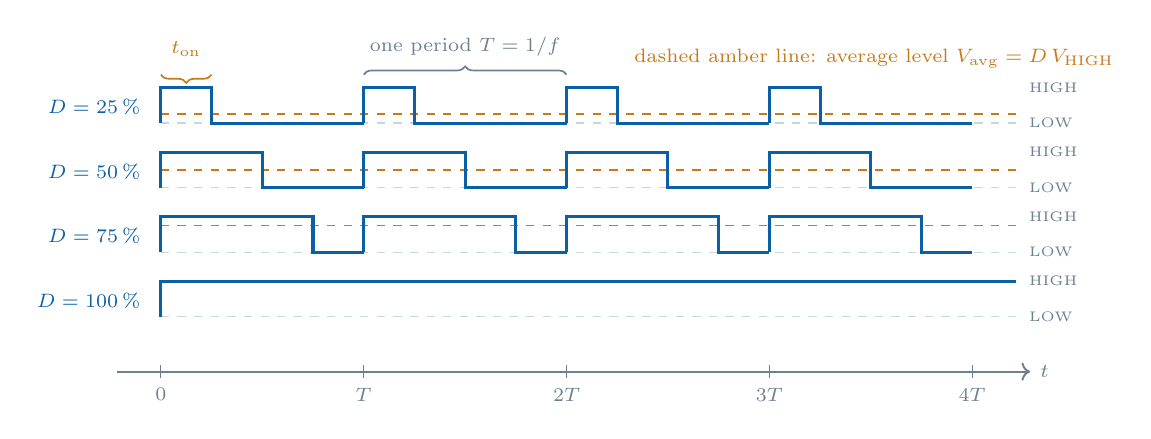
\begin{tikzpicture}[x=0.92cm, y=0.82cm]
  % time axis
  \draw[->, cmnt, line width=0.7pt] (0,-0.55) -- (12.6,-0.55)
        node[right, font=\scriptsize, text=cmnt] {$t$};
  \foreach \x/\lab in {0.6/0, 3.4/$T$, 6.2/$2T$, 9.0/$3T$, 11.8/$4T$}{
      \draw[cmnt] (\x,-0.45) -- (\x,-0.65);
      \node[below, font=\scriptsize, text=cmnt] at (\x,-0.65) {\lab};}
  % four duty cycles: 25 %, 50 %, 75 %, 100 %   (period = 2.8 units)
  \foreach \i/\y/\d/\lab/\avg in {1/3.3/0.7/25\,\%/0.25, 2/2.3/1.4/50\,\%/0.5,
                                  3/1.3/2.1/75\,\%/0.75, 4/0.3/2.8/100\,\%/1}{
    \node[anchor=east, font=\scriptsize\bfseries, text=accent, align=right]
          at (0.45,\y+0.25) {$D=\lab$};
    \draw[rule, dashed, line width=0.4pt] (0.6,\y) -- (12.4,\y);
    \draw[amber, dashed, line width=0.5pt] (0.6,\y+0.55*\avg) -- (12.4,\y+0.55*\avg);
    \pgfmathparse{\d<2.8}
    \ifnum\pgfmathresult=1
      \foreach \k in {0,1,2,3}{
        \pgfmathsetmacro{\xa}{0.6+2.8*\k}
        \pgfmathsetmacro{\xb}{\xa+\d}
        \pgfmathsetmacro{\xc}{\xa+2.8}
        \pgfmathsetmacro{\xe}{min(\xc,12.4)}
        \pgfmathsetmacro{\xf}{min(\xb,12.4)}
        \draw[accent, line width=1.1pt]
          (\xa,\y) -- (\xa,\y+0.55) -- (\xf,\y+0.55) -- (\xf,\y) -- (\xe,\y);}
    \else
      \draw[accent, line width=1.1pt] (0.6,\y) -- (0.6,\y+0.55) -- (12.4,\y+0.55);
    \fi
    \node[font=\tiny, text=cmnt, anchor=west] at (12.45,\y+0.55) {HIGH};
    \node[font=\tiny, text=cmnt, anchor=west] at (12.45,\y) {LOW};}
  % t_on and T brackets on the first waveform
  \draw[decorate, decoration={brace, amplitude=3pt, mirror}, amber, line width=0.6pt]
        (0.6,4.05) -- (1.3,4.05) node[midway, above=3pt, font=\scriptsize, text=amber] {$t_{\mathrm{on}}$};
  \draw[decorate, decoration={brace, amplitude=3pt}, cmnt, line width=0.6pt]
        (3.4,4.05) -- (6.2,4.05) node[midway, above=3pt, font=\scriptsize, text=cmnt] {one period $T=1/f$};
  \node[font=\scriptsize, text=amber, anchor=west] at (7.0,4.3) {dashed amber line: average level $V_{\mathrm{avg}} = D\,V_{\mathrm{HIGH}}$};
\end{tikzpicture}
\caption{PWM waveforms at four duty cycles. The period $T$ is the same in every row;
only the HIGH fraction changes, and with it the average voltage seen by the LED.}
\label{fig:pwm-theory}
\end{figure}

On the Raspberry Pi, \texttt{RPi.GPIO} provides PWM on any GPIO pin in software: a
\texttt{GPIO.PWM(pin, frequency)} object is created for the pin, started with
\texttt{start(duty)}, and its duty cycle can be changed at any time with
\texttt{ChangeDutyCycle(duty)} in the range $0$--$100$. The library toggles the pin from
a background thread, so eight independent PWM channels can run at once --- which is what
this experiment needs, since the Pi has only two hardware PWM channels.

\begin{notebox}
\textbf{Note on current limiting.} As in the earlier experiments, the LEDs were
connected \emph{directly} to the GPIO pins, without series resistors, and the
demonstration ran without damage. PWM does not change the peak current --- during each
ON interval the pin sources the same current as a steadily HIGH pin --- so the usual
advice still applies: a series resistor of roughly $220\,\Omega$ per LED, giving
$(3.3-2)/220 \approx 6\,\mathrm{mA}$, is the recommended practice for sustained use.
\end{notebox}

%------------------------------------------------------------------ 2. MATERIALS
\Needspace{8\baselineskip}
\section{Materials Required}

\noindent
\begin{tabularx}{\textwidth}{@{}p{0.4cm} >{\raggedright\arraybackslash}p{5.2cm} c X@{}}
\toprule
\rowcolor{soft}
\multicolumn{1}{@{}l}{\textbf{\#}} & \textbf{Component} & \textbf{Qty.} & \textbf{Purpose in the setup} \\
\midrule
1 & Raspberry Pi (with SD card, OS installed) & 1 & Host board; generates the eight PWM signals \\
2 & Solderless breadboard                     & 1 & Mounting the LEDs and the ground rail \\
3 & LEDs (5\,mm, red)                         & 8 & One per PWM channel \\
4 & Male--female jumper wires                 & 9--12 & GPIO header to breadboard connections \\
5 & USB power supply                          & 1 & Powering the Raspberry Pi \\
6 & Monitor, keyboard and mouse               & 1 & Running the programs from the terminal \\
\bottomrule
\end{tabularx}

%------------------------------------------------------------------ 3. METHODOLOGY
\section{Methodology}

Eight LEDs were mounted on the breadboard in two columns of four, each anode wired
directly to its own GPIO pin of the Raspberry Pi and all cathodes tied to a common
ground rail returned to a GND pin of the board. The eight pins were configured as
outputs and a software PWM object was created on each, all at the same switching
frequency and all started at $0\,\%$ duty cycle so that the display begins dark.

The experiment was then run in two parts. In \textbf{Part A} the duty cycles were held
constant: four LEDs at $100\,\%$ and the other four at $10\,\%$, giving a direct
side-by-side comparison of a bright group and a dim group driven by the same kind of
signal. In \textbf{Part B} the duty cycle of every channel was recomputed twenty times a
second so that each LED fades smoothly up to full brightness and back down, with the
eight channels offset in time, producing a wave of brightness that travels along the
array.

\subsection{GPIO connections}

\vspace{2pt}
\noindent
\begin{minipage}[t]{0.48\textwidth}
\vspace{0pt}
\begin{tabularx}{\linewidth}{@{}l l >{\raggedright\arraybackslash}X@{}}
\toprule
\rowcolor{soft}
\textbf{LED} & \textbf{Raspberry Pi pin} & \textbf{Part A duty cycle} \\
\midrule
LED 1 & Pin 40 & $100\,\%$ (bright group) \\
LED 2 & Pin 38 & $100\,\%$ \\
LED 3 & Pin 36 & $100\,\%$ \\
LED 4 & Pin 35 & $100\,\%$ \\
LED 5 & Pin 33 & $10\,\%$ (dim group) \\
LED 6 & Pin 32 & $10\,\%$ \\
LED 7 & Pin 31 & $10\,\%$ \\
LED 8 & Pin 29 & $10\,\%$ \\
\midrule
All cathodes & GND & --- \\
\bottomrule
\end{tabularx}
\end{minipage}\hfill
\begin{minipage}[t]{0.49\textwidth}
\vspace{0pt}
\begin{titledbox}[unbreakable]{Numbering used here}
\raggedright
The programs use \textbf{BOARD} numbering (\texttt{GPIO.setmode(GPIO.BOARD)}), so the
numbers in the table are the \emph{physical} positions on the 40-pin header rather than
the Broadcom channel numbers. The same eight pins and the same wiring were used as for
the binary display of Experiment 2; only the software changed. All eight channels
share one switching frequency of $200\,\mathrm{Hz}$, so the only thing that differs
between LEDs is the duty cycle.
\end{titledbox}
\end{minipage}

\begin{figure}[htb]
\centering
\pwmschematiceight{Raspberry Pi}{Pin 40}{Pin 38}{Pin 36}{Pin 35}{Pin 33}{Pin 32}{Pin 31}{Pin 29}
\caption{Circuit schematic. Eight LEDs are driven directly from eight GPIO pins, each
carrying its own software-generated PWM signal, with all cathodes returned to the
common ground rail on the breadboard.}
\label{fig:schematic}
\end{figure}

\subsection{Part A --- two fixed duty cycles}

The first program simply sets and holds the duty cycles: the first four channels at
$100\,\%$ and the last four at $10\,\%$. Because every channel is switched at the same
$200\,\mathrm{Hz}$, any difference in brightness between the two groups can only come
from the duty cycle. At $100\,\%$ the pin is HIGH continuously and the LED is at full
brightness; at $10\,\%$ it is HIGH for only $0.5\,\mathrm{ms}$ of every $5\,\mathrm{ms}$
period, so the LED receives one-tenth of the average current and glows visibly but
much more dimly.

\subsection{Part B --- a travelling wave of brightness}

The second program recomputes every duty cycle on a fixed schedule. Each LED follows the
same cycle of length $6.4\,\mathrm{s}$: its duty cycle rises linearly from $0$ to
$100\,\%$ over $1.6\,\mathrm{s}$, falls back to $0$ over the next $1.6\,\mathrm{s}$, and
stays at $0$ for the remaining $3.2\,\mathrm{s}$. Consecutive LEDs start this cycle
$0.8\,\mathrm{s}$ apart, so the fade runs along the array like a wave. Since each LED is
lit for exactly half its cycle and the eight start times span one full cycle, exactly
four LEDs are lit at any instant: the newest is brightening, the oldest is dimming, and
every $0.8\,\mathrm{s}$ one LED switches off as the next switches on.

\begin{figure}[H]
\centering
\begin{tikzpicture}
\begin{groupplot}[
  group style={group size=1 by 8, vertical sep=2.5pt, x descriptions at=edge bottom},
  width=0.9\textwidth, height=0.95cm, scale only axis,
  xmin=0, xmax=9.6, ymin=0, ymax=112,
  xtick={0,0.8,1.6,2.4,3.2,4.0,4.8,5.6,6.4,7.2,8.0,8.8,9.6},
  xticklabels={0,0.8,1.6,2.4,3.2,4.0,4.8,5.6,6.4,7.2,8.0,8.8,9.6},
  ytick=\empty,
  tick label style={font=\scriptsize, color=cmnt},
  axis line style={rule, line width=0.4pt},
  xmajorgrids, grid style={rule, line width=0.3pt},
  tick style={rule},
  xlabel={time (s)}, xlabel style={font=\scriptsize, color=cmnt},
  every axis plot/.append style={accent, line width=0.8pt},
  clip=false]
\pgfplotsinvokeforeach{1,...,8}{
  \nextgroupplot
  \addplot[fill=accentlt, draw=accent, line width=0.8pt]
    table[x=t, y=LED#1, col sep=comma]{figures/pwm_wave_program.csv} \closedcycle;
  \node[anchor=east, font=\scriptsize\bfseries, text=accent] at (rel axis cs:-0.01,0.5) {LED #1};
}
\end{groupplot}
\node[anchor=south, font=\scriptsize, text=cmnt] at ($(group c1r1.north)+(0,2pt)$)
     {duty cycle of each channel, $0$ to $100\,\%$ (LED 1 starts at $t=0$, each next LED $0.8\,$s later)};
\end{tikzpicture}
\caption{Programmed duty cycle of the eight channels in Part B. Each channel repeats a
$6.4\,\mathrm{s}$ cycle --- fade in, fade out, then dark --- and neighbouring channels are
staggered by $0.8\,\mathrm{s}$, so four LEDs are lit at any moment and the pattern
advances one LED every $0.8\,\mathrm{s}$.}
\label{fig:wave-theory}
\end{figure}

\subsection{Procedure}

\noindent
\begin{minipage}[t]{0.6\textwidth}
\vspace{0pt}
\begin{enumerate}
  \item Eight LEDs were placed on the breadboard in two columns of four, with all
        cathodes on the common ground rail, which was returned to a GND pin of the
        Raspberry Pi.
  \item Each anode was wired to its own GPIO pin in the order given in the table above.
        The wiring was checked with the board powered off.
  \item In the program, the eight pins were configured as outputs and a
        \texttt{GPIO.PWM} object was created for each at $200\,\mathrm{Hz}$ and started
        at $0\,\%$ duty cycle.
  \item \textbf{Part A:} the first four channels were set to $100\,\%$ and the last four
        to $10\,\%$ with \texttt{ChangeDutyCycle()}, and the two groups were compared
        side by side while the program held the values.
  \item \textbf{Part B:} the second program was run. Every $20\,\mathrm{ms}$ it computed
        the position of each channel within its $6.4\,\mathrm{s}$ cycle, converted that
        to a duty cycle with the fade-in/fade-out profile of Figure~\ref{fig:wave-theory},
        and applied it to the channel.
  \item Both runs were recorded on video. The stills in this report are frames from
        those recordings, and the timing of the wave was checked by reading the
        brightness of each LED off the frames.
  \item Finally, on \texttt{Ctrl+C}, every PWM channel was stopped with
        \texttt{stop()} and \texttt{GPIO.cleanup()} returned all the pins to inputs.
\end{enumerate}
\end{minipage}\hfill
\begin{minipage}[t]{0.36\textwidth}
\vspace{0pt}
\centering
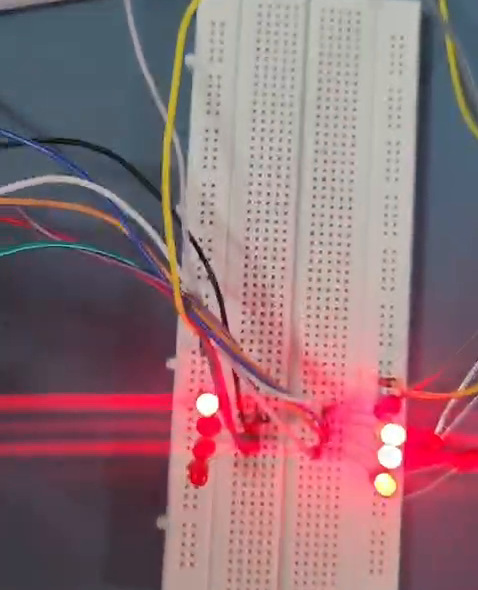
\includegraphics[width=0.88\linewidth]{figures/pwm_setup.jpg}
\captionof{figure}{The assembled circuit --- eight LEDs in two columns of four on the
breadboard, each wired directly to its own GPIO pin through the bundle of jumper wires
running to the Raspberry Pi's header (off the top of the frame), with the cathodes on
the common ground rail.}
\label{fig:setup}
\end{minipage}

\Needspace{40\baselineskip}
\subsection{Code (Python, Raspberry Pi)}

\begin{lstlisting}[language=Python, caption={Part A --- two groups of LEDs held at two fixed duty cycles.}, label={lst:levels}]
import RPi.GPIO as GPIO
import time

# Physical (BOARD) pin numbers of the eight LEDs, LED 1 first
LED_PINS = [40, 38, 36, 35, 33, 32, 31, 29]
PWM_FREQ = 200          # switching frequency in Hz, well above flicker

DUTY_BRIGHT = 100       # LEDs 1-4: full brightness
DUTY_DIM    = 10        # LEDs 5-8: one tenth of the average current

GPIO.setmode(GPIO.BOARD)
GPIO.setwarnings(False)

pwm = []
for pin in LED_PINS:
    GPIO.setup(pin, GPIO.OUT, initial=GPIO.LOW)
    channel = GPIO.PWM(pin, PWM_FREQ)   # one software PWM channel per pin
    channel.start(0)                    # begin with the LED off
    pwm.append(channel)
try:
    for channel in pwm[:4]:
        channel.ChangeDutyCycle(DUTY_BRIGHT)
    for channel in pwm[4:]:
        channel.ChangeDutyCycle(DUTY_DIM)
    print("LEDs 1-4 at", DUTY_BRIGHT, "% | LEDs 5-8 at", DUTY_DIM, "%")

    while True:
        time.sleep(1)                   # hold the levels until Ctrl+C

except KeyboardInterrupt:
    print("\nExiting program")

finally:
    for channel in pwm:
        channel.stop()
    GPIO.cleanup()
\end{lstlisting}

\Needspace{14\baselineskip}
\begin{lstlisting}[language=Python, caption={Part B --- a wave of brightness travelling along the eight LEDs.}, label={lst:wave}]
import RPi.GPIO as GPIO
import time

LED_PINS = [40, 38, 36, 35, 33, 32, 31, 29]
PWM_FREQ = 200          # Hz
CYCLE    = 6.4          # s, one fade-in / fade-out / dark cycle of an LED
STAGGER  = CYCLE / 8    # 0.8 s between the start of neighbouring LEDs
TICK     = 0.02         # s between duty-cycle updates

def duty_cycle(phase):
    """Duty cycle (0-100 %) for a position in the cycle, phase in [0, 1)."""
    if phase < 0.25:                      # fade in over the first quarter
        return 100 * phase / 0.25
    if phase < 0.5:                       # fade out over the second quarter
        return 100 * (0.5 - phase) / 0.25
    return 0                              # dark for the second half

GPIO.setmode(GPIO.BOARD)
GPIO.setwarnings(False)
pwm = []
for pin in LED_PINS:
    GPIO.setup(pin, GPIO.OUT, initial=GPIO.LOW)
    channel = GPIO.PWM(pin, PWM_FREQ)
    channel.start(0)
    pwm.append(channel)
try:
    t0 = time.time()
    while True:
        t = time.time() - t0
        for i, channel in enumerate(pwm):
            phase = ((t - i * STAGGER) / CYCLE) % 1.0
            channel.ChangeDutyCycle(duty_cycle(phase))
        time.sleep(TICK)

except KeyboardInterrupt:
    print("\nExiting program")

finally:
    for channel in pwm:
        channel.stop()
    GPIO.cleanup()
\end{lstlisting}

%------------------------------------------------------------------ 4. RESULT
\section{Result and Output}

\begin{keybox}
Both parts worked as intended. In \textbf{Part A} the four LEDs at $100\,\%$ duty cycle
glowed at full brightness while the four at $10\,\%$ were clearly lit but much dimmer,
with no other difference between the groups. In \textbf{Part B} the LEDs faded up and
down in turn: \textbf{four were lit at any moment}, the pattern advanced by one LED every
$0.8\,\mathrm{s}$, and each LED was lit for $3.2\,\mathrm{s}$ and dark for
$3.2\,\mathrm{s}$ --- a $6.4\,\mathrm{s}$ cycle, exactly as programmed.
\end{keybox}

\subsection*{Observed outputs}

\vspace{2pt}
\noindent
\begin{tabularx}{\textwidth}{@{}c l l X@{}}
\toprule
\rowcolor{soft}
\textbf{Output} & \textbf{Run} & \textbf{Duty cycle set} & \textbf{What was observed} \\
\midrule
1 & Part A, LEDs 1--4 & $100\,\%$ (held) & full brightness; the four LEDs of one
      column glow steadily with bright white centres in the video \\
2 & Part A, LEDs 5--8 & $10\,\%$ (held) & clearly lit but much dimmer; the four LEDs
      of the other column show only a red glow, no bright centre \\
3 & Part B, all eight & $0\to100\to0\,\%$, staggered & a wave of brightness travels
      along the LEDs; four lit at a time, advancing one LED every $0.8\,\mathrm{s}$
      (measured from the video, Figure~\ref{fig:wave-measured}) \\
\bottomrule
\end{tabularx}

\vspace{8pt}
\noindent In Part A the switching frequency was identical for both groups, so the
difference in brightness is due to the duty cycle alone. In Part B the timing read off
the video --- one LED switching on and one switching off every $0.8\,\mathrm{s}$, each LED
lit for $3.2\,\mathrm{s}$ --- matches the constants \texttt{STAGGER = 0.8} and
\texttt{CYCLE / 2 = 3.2} in Listing~\ref{lst:wave}.

\subsection*{Part A --- two fixed duty cycles}

\vspace{2pt}
\noindent
\begin{minipage}[t]{0.485\textwidth}
\centering
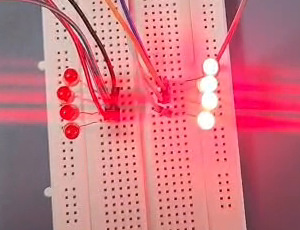
\includegraphics[width=\linewidth]{figures/pwm_two_levels_a.jpg}
\end{minipage}\hfill
\begin{minipage}[t]{0.485\textwidth}
\centering
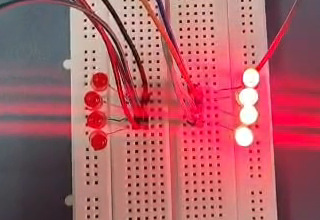
\includegraphics[width=\linewidth]{figures/pwm_two_levels_b.jpg}
\end{minipage}
\captionof{figure}{Part A, two frames from the recording. The right-hand column of four
LEDs is driven at $100\,\%$ duty cycle and the left-hand column at $10\,\%$. Both groups
are lit, but the $10\,\%$ group is visibly dimmer --- the camera shows only the red glow
of the LED body, without the bright centre of the $100\,\%$ group.}
\label{fig:levels}

\subsection*{Part B --- the travelling wave}

\begin{figure}[H]
\centering
\begin{minipage}[t]{0.45\textwidth}
\centering
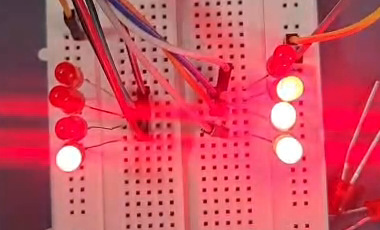
\includegraphics[width=\linewidth]{figures/pwm_wave_t1.jpg}\\[2pt]
{\scriptsize\color{cmnt} $t = 0.5\,\mathrm{s}$}
\end{minipage}\hfill
\begin{minipage}[t]{0.45\textwidth}
\centering
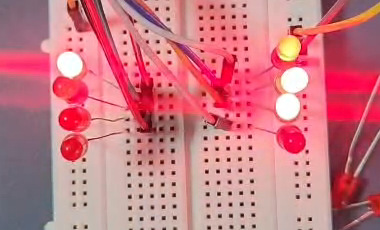
\includegraphics[width=\linewidth]{figures/pwm_wave_t2.jpg}\\[2pt]
{\scriptsize\color{cmnt} $t = 1.9\,\mathrm{s}$}
\end{minipage}

\vspace{6pt}
\begin{minipage}[t]{0.45\textwidth}
\centering
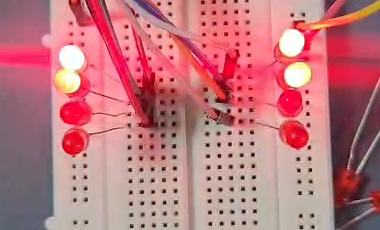
\includegraphics[width=\linewidth]{figures/pwm_wave_t3.jpg}\\[2pt]
{\scriptsize\color{cmnt} $t = 2.9\,\mathrm{s}$}
\end{minipage}\hfill
\begin{minipage}[t]{0.45\textwidth}
\centering
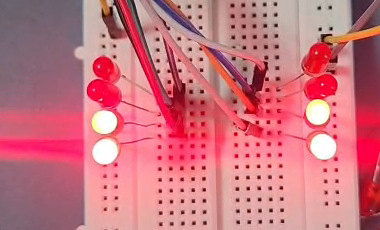
\includegraphics[width=\linewidth]{figures/pwm_wave_t4.jpg}\\[2pt]
{\scriptsize\color{cmnt} $t = 6.0\,\mathrm{s}$}
\end{minipage}
\caption{Part B at four instants of the same recording. In every frame four
LEDs are lit. The LED that has just switched on is still brightening --- it appears
yellowish rather than white, since its duty cycle is still rising --- while the LED
about to switch off is dimming; the fully bright ones in between are at or near
$100\,\%$. Comparing the frames shows the lit group moving through the array.}
\label{fig:wave-photos}
\end{figure}

\begin{figure}[H]
\centering
\begin{tikzpicture}
\begin{groupplot}[
  group style={group size=1 by 8, vertical sep=2.5pt, x descriptions at=edge bottom},
  width=0.9\textwidth, height=0.8cm, scale only axis,
  xmin=0, xmax=7.2, ymin=0, ymax=105,
  xtick={0,0.8,1.6,2.4,3.2,4.0,4.8,5.6,6.4,7.2},
  xticklabels={0,0.8,1.6,2.4,3.2,4.0,4.8,5.6,6.4,7.2},
  ytick=\empty,
  tick label style={font=\scriptsize, color=cmnt},
  axis line style={rule, line width=0.4pt},
  xmajorgrids, grid style={rule, line width=0.3pt},
  tick style={rule},
  xlabel={time in the recording (s)}, xlabel style={font=\scriptsize, color=cmnt},
  every axis plot/.append style={accent, line width=0.8pt},
  clip=false]
\pgfplotsinvokeforeach{R2,L1,R1,L2,L3,L4,R4,R3}{
  \nextgroupplot
  \addplot[fill=accentlt, draw=accent, line width=0.8pt]
    table[x=t, y=#1, col sep=comma]{figures/led_brightness.csv} \closedcycle;
  \node[anchor=east, font=\scriptsize\bfseries, text=accent] at (rel axis cs:-0.01,0.5) {#1};
}
\end{groupplot}
\node[anchor=south, font=\scriptsize, text=cmnt] at ($(group c1r1.north)+(0,2pt)$)
     {brightness of each LED read from the video frames (20 frames per second), $0$ to $100\,\%$ of the camera's full scale};
\end{tikzpicture}
\caption{Part B, measured. The brightness of each LED was read from the video frames
(the average green-channel value of the pixels covering the LED, which is the camera
channel that saturates last) for the first $7.2\,\mathrm{s}$ of the recording.
L and R denote the left and right columns of LEDs on the breadboard, numbered from
the top; the panels are ordered by the time each LED switched on, which follows the
program's pin order rather than the LEDs' physical positions. Each LED is lit for
$3.2\,\mathrm{s}$ and dark for $3.2\,\mathrm{s}$, and successive LEDs switch on
$0.8\,\mathrm{s}$ apart --- the same pattern as Figure~\ref{fig:wave-theory}. The camera
saturates well below full brightness, which is why the fade-in and fade-out ramps of
the programmed triangle appear as plateaus with short edges here.}
\label{fig:wave-measured}
\end{figure}

\subsection*{Video demonstration and code}

\begin{titledbox}[before skip=6pt]{Google Drive link}
\noindent The demonstration videos, this report and the complete source code are
available in the following shared folder:

\vspace{4pt}
\noindent\drivefolder

\vspace{4pt}
{\small\color{cmnt} Access has been set to \emph{anyone with the link can view}.}
\end{titledbox}

\subsection*{Discussion}
\label{sec:discussion}
\begin{itemize}
  \item \textbf{Software PWM.} \texttt{RPi.GPIO} generates each PWM signal from a
        Python-level thread, so the timing is not as precise as hardware PWM and can
        jitter when the processor is busy. At $200\,\mathrm{Hz}$ with eight channels this
        was not visible to the eye, but it is why hardware PWM (available on only two
        channels of the Pi) is preferred where the exact frequency matters, for example
        for servo control.
  \item \textbf{The camera sees PWM differently from the eye.} In the Part A recording
        the bright group occasionally appears to dip for a frame or two at regular
        intervals. This is a beat between the $200\,\mathrm{Hz}$ switching and the
        camera's frame rate and rolling shutter, not a change in the programmed duty
        cycle: to the eye the brightness was steady. Likewise, the camera saturates at a
        duty cycle well below $100\,\%$, which is why the smooth triangular fades of
        Part B come out as near-square pulses in Figure~\ref{fig:wave-measured}.
  \item \textbf{Perceived brightness is not linear in duty cycle.} The eye responds
        roughly logarithmically to light, so the step from $10\,\%$ to $100\,\%$ looks
        smaller than a factor of ten, and most of the visible change in a linear fade
        happens at the low end. A fade that looks uniform would use a duty cycle that
        rises exponentially (or as a square) rather than linearly.
  \item \textbf{Frequency and flicker.} At $200\,\mathrm{Hz}$ no flicker was visible at any
        duty cycle. At a much lower frequency (a few tens of hertz) the same program would
        show visible flicker at low duty cycles, and at $1$--$2\,\mathrm{Hz}$ the PWM signal
        becomes the blinking of Experiment~1 --- PWM is simply that blinking made fast
        enough to blur into a steady brightness.
  \item \textbf{Current.} PWM reduces the \emph{average} current but not the peak, so
        driving the LEDs without series resistors carries the same risk as before, and a
        $220\,\Omega$ resistor per LED remains the safer arrangement.
\end{itemize}

%------------------------------------------------------------------ CONCLUSION
\Needspace{12\baselineskip}
\section{Conclusion}

The experiment showed how a purely digital output can be made to behave like an
adjustable one. By switching each GPIO pin rapidly and controlling only the fraction of
time it spends HIGH, the Raspberry Pi set the brightness of eight LEDs independently:
two fixed duty cycles produced two clearly different, steady brightness levels, and
sweeping the duty cycles continuously in software produced a smooth wave of brightness
travelling along the array, with four LEDs lit at a time and the pattern advancing every
$0.8\,\mathrm{s}$, exactly as programmed.

Where Experiment~1 used GPIO to switch LEDs and Experiment~2 used a group of pins as a
parallel binary port, this experiment used time --- the duty cycle --- as the controlled
quantity. The same technique extends directly to dimming lamps, driving motors at
variable speed, and positioning servos, all of which are controlled with PWM from GPIO
pins in the same way.

\end{document}
